% =====================================================================
%  FoodGenome AI — presentation
%
%  Build:  ./build.sh    (or: tectonic slides.tex)
%
%  Figures are shared with the paper rather than duplicated, so the two can
%  never disagree about a number.
% =====================================================================

\documentclass[aspectratio=169,11pt]{beamer}

\newcommand{\StudentName}{A K M Asifuzzaman}
\newcommand{\CourseCode}{CSE 450 Python Project}

\usetheme{default}
\usecolortheme{default}
\usefonttheme{professionalfonts}

\usepackage[T1]{fontenc}
\usepackage{lmodern}
\usepackage{microtype}
\usepackage{graphicx}
\usepackage{xcolor}
\usepackage{booktabs}

\graphicspath{{../paper/figures/}}

\definecolor{ink}{RGB}{11,11,15}
\definecolor{comicred}{RGB}{230,36,41}
\definecolor{comicblue}{RGB}{27,76,224}
\definecolor{newsprint}{RGB}{244,241,232}
\definecolor{dim}{RGB}{75,75,85}
\definecolor{good}{RGB}{22,163,74}

\setbeamercolor{normal text}{fg=ink,bg=newsprint}
\setbeamercolor{frametitle}{fg=ink,bg=}
\setbeamercolor{structure}{fg=comicred}
\setbeamercolor{alerted text}{fg=comicred}
\setbeamerfont{frametitle}{series=\bfseries,size=\large}
\setbeamertemplate{navigation symbols}{}
\setbeamertemplate{itemize item}{\color{comicred}\textbf{--}}
\setbeamertemplate{itemize subitem}{\color{dim}\textbf{\textperiodcentered}}

% A hairline under every frame title, which is the one piece of the comic
% language that survives being shrunk to slide scale.
\setbeamertemplate{frametitle}{%
  \vspace{0.5em}\insertframetitle\par
  \vspace{-0.35em}{\color{ink}\rule{\textwidth}{1.1pt}}\par\vspace{-0.3em}}

\setbeamertemplate{footline}{%
  \hfill\scriptsize\color{dim}\insertframenumber\hspace{1.2em}\vspace{0.6em}}

\newcommand{\headline}[2]{%
  {\Huge\bfseries\color{comicred}#1}\\[0.15em]{\normalsize\color{dim}#2}}

\title{FoodGenome AI}
\author{\StudentName}

\begin{document}

% ── 1 ────────────────────────────────────────────────────────────────
\begin{frame}[plain]
\vspace{1.2em}
{\Huge\bfseries FoodGenome AI}\\[0.5em]
{\large Calibrated food recognition with conformal guarantees\\and grounded nutritional retrieval}\\[1.6em]
{\color{dim}\itshape What five negative results taught us about\\when added complexity does not pay}\\[2em]
{\small \StudentName \quad\textbullet\quad \CourseCode}\\[0.4em]
{\scriptsize\color{dim} food-red-omega.vercel.app}
\end{frame}

% ── 2 ────────────────────────────────────────────────────────────────
\begin{frame}{The problem}
\begin{columns}[T]
\begin{column}{0.55\textwidth}
Photograph a dish. The system returns:
\begin{itemize}
  \item the category, from 101
  \item a confidence that \emph{means} something
  \item every candidate it cannot rule out
  \item nutrition traced to a USDA record
\end{itemize}
\vspace{0.8em}
And, when it should:
\begin{itemize}
  \item[] \alert{nothing at all}
\end{itemize}
\end{column}
\begin{column}{0.42\textwidth}
\vspace{0.5em}
{\color{dim}\small
A nutrition figure shown without qualification will be acted on.

A classifier restricted to 101 categories will return one of them for a photograph of a car.

\vspace{0.6em}
So \textbf{knowing when not to answer} is a requirement, not a nicety.}
\end{column}
\end{columns}
\end{frame}

% ── 3 ────────────────────────────────────────────────────────────────
\begin{frame}{Headline}
\vspace{0.4em}
\begin{columns}[T]
\begin{column}{0.24\textwidth}\centering
\headline{97.16\%}{Food-101 test top-1\\on a sealed split}
\end{column}
\begin{column}{0.24\textwidth}\centering
\headline{99.56\%}{conformal coverage\\1.54 candidates}
\end{column}
\begin{column}{0.24\textwidth}\centering
\headline{97.94\%}{on accepted images\\after abstaining on 2.3\%}
\end{column}
\begin{column}{0.24\textwidth}\centering
\headline{98.6\%}{RAG answers correct\\100\% grounded}
\end{column}
\end{columns}
\vspace{1.6em}
{\color{dim} Validation is a fixed 4\% stratified slice carved from \emph{train}, seed 1337.
The 25{,}250-image test split was untouched until final evaluation --- and the mask was
hashed and verified before the fine-tune on separate hardware was allowed to start.}
\end{frame}

% ── 4 ────────────────────────────────────────────────────────────────
\begin{frame}{Method}
\begin{columns}[T]
\begin{column}{0.48\textwidth}
\textbf{Vision}
\begin{itemize}
  \item Three backbones run once, embeddings cached (\textasciitilde20 h)
  \item Every later experiment then takes \emph{seconds}
  \item Small MLP heads, probability average
\end{itemize}
\vspace{0.7em}
\textbf{Reliability}
\begin{itemize}
  \item Temperature fitted on held-out data
  \item Split-conformal prediction sets
  \item Abstention on two signals
\end{itemize}
\end{column}
\begin{column}{0.48\textwidth}
\textbf{Knowledge}
\begin{itemize}
  \item 101 classes $\times$ 32 USDA nutrients
  \item BM25 + bi-encoder, fused by RRF
  \item Cross-encoder rerank
  \item Query rewritten with the predicted dish
\end{itemize}
\vspace{0.7em}
\textbf{Grounding}
\begin{itemize}
  \item Every number verified against a source
  \item Matched \emph{per unit}
  \item Failures withheld, not annotated
\end{itemize}
\end{column}
\end{columns}
\end{frame}

% ── 5 ────────────────────────────────────────────────────────────────
\begin{frame}{The caching decision made rigour affordable}
\vspace{0.5em}
{\large Running each backbone once and caching the embeddings cost twenty hours.}
\vspace{1em}

Every question afterwards became cheap:
\begin{itemize}
  \item head architecture
  \item calibration, conformal sets, abstention thresholds
  \item \textbf{every ensemble combination} --- rerun dozens of times
\end{itemize}
\vspace{1em}
{\color{dim} Without the cache each of those reruns would have been a fresh forward pass over
101{,}000 images. The ablation on the next slides simply would not have been affordable.}
\end{frame}

% ── 6 ────────────────────────────────────────────────────────────────
\begin{frame}{Negative result 1 --- a trained head lost to arithmetic}
\begin{columns}[T]
\begin{column}{0.56\textwidth}
\vspace{-0.4em}
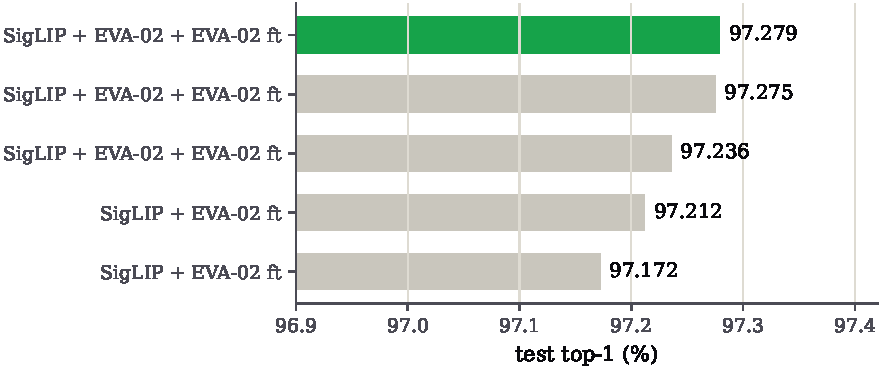
\includegraphics[width=\textwidth]{ablation_slide.pdf}
\end{column}
\begin{column}{0.40\textwidth}
\vspace{0.6em}
A gated fusion head:
\begin{itemize}
  \item 3.97M parameters
  \item 21.9 minutes of training
  \item \textbf{96.97\%}
\end{itemize}
\vspace{0.5em}
A 50/50 average:
\begin{itemize}
  \item 0 parameters
  \item milliseconds
  \item \alert{\textbf{97.16\%}}
\end{itemize}
\vspace{0.7em}
{\small McNemar: the average wins at $p=0.005$. The fusion head does \emph{not} beat its own
best input ($p=0.071$).}
\end{column}
\end{columns}
\end{frame}

% ── 7 ────────────────────────────────────────────────────────────────
\begin{frame}{Negative result 2 --- the third backbone earned no place}
\vspace{0.6em}
DINOv2-L is the only \textbf{self-supervised} member, so it was predicted to make the most
independent errors.
\vspace{1em}

It makes the least:
\vspace{0.4em}
\begin{center}\small
\begin{tabular}{lr}
\toprule
Share of SigLIP's errors also made by\dots & \\
\midrule
EVA-02-L (supervised) & 65.2\% \\
DINOv2-L (self-supervised) & \alert{66.3\%} \\
\bottomrule
\end{tabular}
\end{center}
\vspace{1em}
Adding it moved the ensemble to 97.09\% --- marginally \emph{below} the pair, at $p=0.312$.
A weight search on validation independently drove its weight to \textbf{0.05}.
\end{frame}

% ── 8 ────────────────────────────────────────────────────────────────
\begin{frame}{Confidence that means something}
\begin{columns}[T]
\begin{column}{0.44\textwidth}
\vspace{-0.3em}
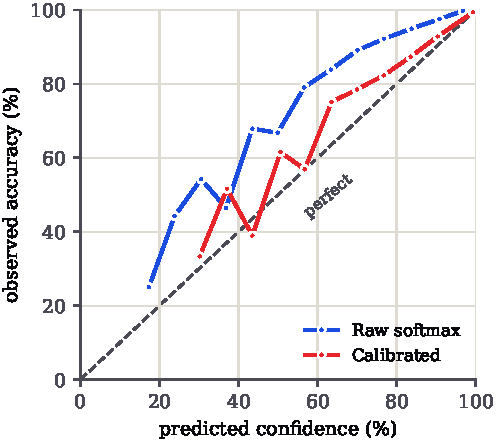
\includegraphics[width=\textwidth]{reliability.pdf}
\end{column}
\begin{column}{0.52\textwidth}
\vspace{0.8em}
The ensemble sat \textbf{above} the diagonal --- systematically \emph{under}-confident, the
less common direction.
\vspace{0.8em}
\begin{center}\small
\begin{tabular}{lrr}
\toprule
 & before & after \\
\midrule
ECE & 0.0514 & \textbf{0.0062} \\
mean confidence & 92.0\% & 96.6\% \\
accuracy & 97.16\% & 97.16\% \\
\bottomrule
\end{tabular}
\end{center}
\vspace{0.6em}
{\small Accuracy is unchanged and must be --- temperature scaling is monotonic. It changes
only what the number \emph{means}.}
\end{column}
\end{columns}
\end{frame}

% ── 9 ────────────────────────────────────────────────────────────────
\begin{frame}{A guarantee, not a feeling}
\vspace{0.4em}
A calibrated confidence is a claim about one image.\\
A \textbf{conformal set} is a claim about the procedure --- and it holds without assuming
anything about the model.
\vspace{0.9em}
\begin{center}\small
\begin{tabular}{lrrr}
\toprule
Target & Method & Coverage & Mean set size \\
\midrule
90\% & LAC & 93.59\% & 0.95 \\
90\% & APS & 90.18\% & 1.54 \\
99\% & LAC + top-1 & \alert{\textbf{99.56\%}} & \textbf{1.54} \\
\bottomrule
\end{tabular}
\end{center}
\vspace{0.9em}
{\color{dim} Below the model's own 97.16\% accuracy the guarantee is met by the single best
guess and the ``set'' degenerates to one class. The machinery only does work at 99\%.}
\end{frame}

% ── 10 ───────────────────────────────────────────────────────────────
\begin{frame}{Negative result 3 --- the broken version looked \emph{better}}
\vspace{0.6em}
An early implementation forced the top-1 class into the set at test time, but scored
\textbf{without} it during calibration.
\vspace{0.9em}

That silently rescued the 13\% of images whose top score exceeded the threshold:
\vspace{0.5em}
\begin{center}
{\large target \textbf{90\%} \quad$\rightarrow$\quad measured \alert{\textbf{99.1\%}}}
\end{center}
\vspace{0.9em}
The guarantee was \textbf{void} --- and the reported number was better for it.
\vspace{0.8em}

{\color{dim} Conformal validity requires the identical rule in calibration and deployment.
A bug that makes your metric worse gets found. One that makes it better does not.}
\end{frame}

% ── 11 ───────────────────────────────────────────────────────────────
\begin{frame}{Negative result 4 --- attention is not saliency}
\begin{columns}[T]
\begin{column}{0.48\textwidth}
\vspace{0.3em}
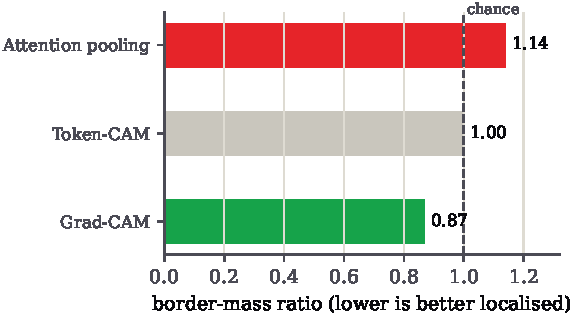
\includegraphics[width=\textwidth]{attribution.pdf}
\vspace{0.3em}
{\scriptsize\color{dim} Share of attribution mass in the outer ring (60\% of the frame),
over 24 test images. Subjects are centred, so lower is better.}
\end{column}
\begin{column}{0.48\textwidth}
\vspace{0.8em}
Reading the pooling head's own attention \emph{should} be the most faithful account of where
the model looked --- those weights are literally the mixture being classified.
\vspace{0.8em}

It is \alert{worse than chance} at finding the food.
\vspace{0.8em}

{\small Reproduces the documented tendency of ViTs to park high attention on
low-information background patches.}
\end{column}
\end{columns}
\end{frame}

% ── 12 ───────────────────────────────────────────────────────────────
\begin{frame}{Negative result 5 --- fine-tuning decorrelated but did not win}
\begin{columns}[T]
\begin{column}{0.44\textwidth}
\vspace{-0.2em}
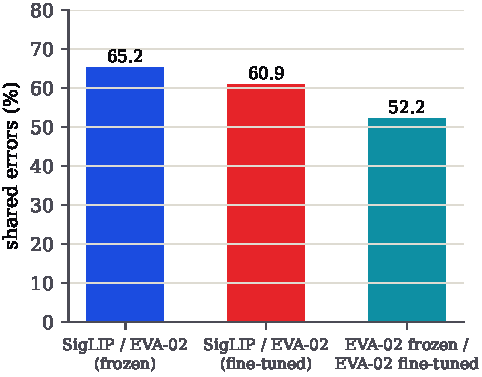
\includegraphics[width=\textwidth]{decorrelation.pdf}
\end{column}
\begin{column}{0.52\textwidth}
\vspace{0.7em}
Nine GPU-hours: 6 epochs at 224\,px, 1 at 448\,px.
\vspace{0.6em}
\begin{itemize}
  \item Alone: 95.90\% --- \emph{below} the pair
  \item At 224\,px: 65.5\% shared errors --- no diversity at all
  \item At 448\,px: \textbf{60.9\%} --- real diversity
\end{itemize}
\vspace{0.7em}
The 448 epoch added \textbf{0.2} points of accuracy and \textbf{4.3} points of diversity.
\vspace{0.6em}

Three-way ensemble: 97.27\%, \alert{$p=0.052$} --- just short.
\end{column}
\end{columns}
\end{frame}

% ── 13 ───────────────────────────────────────────────────────────────
\begin{frame}{Retrieval that refuses}
\begin{columns}[T]
\begin{column}{0.52\textwidth}
\vspace{-0.2em}
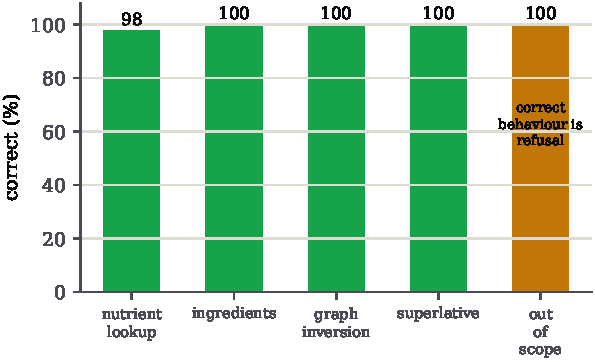
\includegraphics[width=\textwidth]{rag.pdf}
\end{column}
\begin{column}{0.44\textwidth}
\vspace{0.8em}
\begin{itemize}
  \item 98.6\% of in-scope questions correct
  \item \textbf{100\%} refusal accuracy, zero false refusals
  \item 100\% of answers grounded
  \item \$0.024 for the whole evaluation
\end{itemize}
\vspace{0.8em}
{\small Ground truth is \emph{derived} from the knowledge base, not judged by a model --- a
language-model judge shares error modes with the system under test.}
\end{column}
\end{columns}
\end{frame}

% ── 14 ───────────────────────────────────────────────────────────────
\begin{frame}{The grounding gate caught a real one}
\vspace{0.7em}
First live query. Asked for sodium per serving, the model answered:
\vspace{0.6em}
\begin{center}{\Large \textbf{983.4\,mg}}\end{center}
\vspace{0.6em}

That figure is \textbf{arithmetically correct} --- $447 \times 2.2$ --- and the source even
states the multiplier.
\vspace{0.5em}

But it appeared in \emph{no document}, so it was rejected.
\vspace{1em}

{\color{dim}\textbf{The fix went in the corpus, not the tolerance.} The micronutrient
documents stated only per-100\,g, so the model had to multiply to answer at all. Both bases
are now written explicitly.

Loosening the check would have hidden exactly the class of error it exists to catch.}
\end{frame}

% ── 15 ───────────────────────────────────────────────────────────────
\begin{frame}{What it cannot do}
\begin{itemize}
  \item \textbf{Attribution is diffuse} --- 0.87$\times$ chance. The classifier sees a
        globally pooled vector, so position is discarded before it ever sees the image.
  \item \textbf{60 of 101 nutrition profiles are composed} from weighted ingredients, not
        measured. Every surface says which.
  \item \textbf{Abstention is a baseline}, not a trained OOD detector --- it reports the
        model is lost, which is not the same as ``this is not food''.
  \item \textbf{The knowledge base is closed} at 101 categories. Anything else is refused
        rather than estimated.
\end{itemize}
\vspace{0.8em}
{\color{dim} Oracle accuracy --- the ceiling if a perfect combiner always picked a correct
member --- is 98.43\%. Only 1.57\% of test images defeat every model, and much of that is
Food-101's own label noise. This approach is close to exhausted.}
\end{frame}

% ── 16 ───────────────────────────────────────────────────────────────
\begin{frame}{What the negative results have in common}
\vspace{0.8em}
{\large Four of the five share a shape: \textbf{an added component had nothing left to
improve}.}
\vspace{1.2em}
\begin{itemize}
  \item The fusion head had nothing to learn --- two correlated members need no per-input
        weighting.
  \item DINOv2 added no diversity --- self-supervision did not produce independent errors
        here.
  \item Fine-tuning added diversity, but too little to move a 25{,}250-image comparison.
\end{itemize}
\vspace{1.2em}
{\color{dim} Reporting them costs a headline number and buys a defensible account of where
the remaining headroom \emph{is not}.}
\end{frame}

% ── 17 ───────────────────────────────────────────────────────────────
\begin{frame}[plain]
\vspace{2.2em}
\begin{center}
{\Huge\bfseries\color{comicred} Thank you}\\[1.4em]
{\large food-red-omega.vercel.app}\\[0.5em]
{\normalsize github.com/A-K-M-Asifuzzaman/Food}\\[2em]
{\color{dim} \StudentName \quad\textbullet\quad \CourseCode}
\end{center}
\end{frame}

\end{document}
